% ****** Start of file apssamp.tex ******
%
%   This file is part of the APS files in the REVTeX 4.1 distribution.
%   Version 4.1r of REVTeX, August 2010
%
%   Copyright (c) 2009, 2010 The American Physical Society.
%
%   See the REVTeX 4 README file for restrictions and more information.
%
% TeX'ing this file requires that you have AMS-LaTeX 2.0 installed
% as well as the rest of the prerequisites for REVTeX 4.1
%
% See the REVTeX 4 README file
% It also requires running BibTeX. The commands are as follows:
%
%  1)  latex apssamp.tex
%  2)  bibtex apssamp
%  3)  latex apssamp.tex
%  4)  latex apssamp.tex
%
\documentclass[%
 % reprint,
%superscriptaddress,
%groupedaddress,
%unsortedaddress,
%runinaddress,
%frontmatterverbose,
preprint,
%showpacs,preprintnumbers,
%nofootinbib,
%nobibnotes,
%bibnotes,
 amsmath,amssymb,
 aps,
 prd
%pra,
%prb,
%rmp,
%prstab,
%prstper,
%floatfix,
]{revtex4-1}

\usepackage{graphicx}% Include figure files
\usepackage{dcolumn}% Align table columns on decimal point
\usepackage{bm}% bold math
%\usepackage{hyperref}% add hypertext capabilities
%\usepackage[mathlines]{lineno}% Enable numbering of text and display math
%\linenumbers\relax % Commence numbering lines

%\usepackage[showframe,%Uncomment any one of the following lines to test
%%scale=0.7, marginratio={1:1, 2:3}, ignoreall,% default settings
%%text={7in,10in},centering,
%%margin=1.5in,
%%total={6.5in,8.75in}, top=1.2in, left=0.9in, includefoot,
%%height=10in,a5paper,hmargin={3cm,0.8in},
%]{geometry}

\newcommand{\ii}{\mathrm i}


%%%%%%%%%%%%%%%%%%%%%%%%%%%%%%%%%
%%%%% Packages for draft only
%%%%%%%%%%%%%%%%%%%%%%%%%%%%%%%%%%

\usepackage[normalem]{ulem}
\usepackage{xcolor}


\begin{document}

%\preprint{APS/123-QED}

\title{Dispersion Relation Gaps and Neutrino Flavor Instabilities in Fast Modes}% Force line breaks with \\
\thanks{A footnote to the article title}%

\author{Ann Author}
 \altaffiliation[Also at ]{Physics Department, XYZ University.}%Lines break automatically or can be forced with \\
\author{Second Author}%
 \email{Second.Author@institution.edu}
\affiliation{%
 Authors' institution and/or address\\
 This line break forced with \textbackslash\textbackslash
}%


\date{\today}% It is always \today, today,
             %  but any date may be explicitly specified

\begin{abstract}

ABSTRACT PLACEHOLDER


% \begin{description}
% \item[Usage]
% Secondary publications and information retrieval purposes.
% \item[PACS numbers]
% May be entered using the \verb+\pacs{#1}+ command.
% \item[Structure]
% You may use the \texttt{description} environment to structure your abstract;
% use the optional argument of the \verb+\item+ command to give the category of each item.
% \end{description}
\end{abstract}

% \pacs{Valid PACS appear here}% PACS, the Physics and Astronomy
                             % Classification Scheme.
%\keywords{Suggested keywords}%Use showkeys class option if keyword
                              %display desired
\maketitle

%\tableofcontents



\section{\label{sec-introduction}Introduction}


Neutrino flavor conversions in vacuum are linear effects in Schrodinger equation, in other words, the vacuum Hamiltonian doesn't depend on the state of neutrino flavors. However, neutrinos propagate in dense neutrino media demonstrate highly nonlinear flavor transformations due to forward scattering interactions of neutrinos. Such interactions lead to flavor conversions instabilities. The technique used to investigate the nonlinear neutrino flavor conversion is linear stability analysis \cite{Banerjee2011a,Raffelt2013}. Recent studies by I. Izaguirre, G. Raffelt, and I. Tamborra show that linear stability analysis indicates the dispersion relation \cite{Izaguirre2016a}. They also showed that dispersion relation can be defined and calculated in linear regime of neutrino flavor conversions. Moreover, they conclued that neutrino flavor conversion instabilities occur within gaps in dispersion relation. We argue that neutrino flavor conversion instabilities is not exactly mapped to gaps in dispersion relation for discrete emission with more than two angles or continuous angular distributions of neutrino emissions. To begin with, we review reference \onlinecite{Izaguirre2016a} to explain the dispersion relation in Sec. \ref{sec-dr}.



\section{\label{sec-dr}Dispersion Relation of Neutrino Flavor Conversion}

We consider two-flavor scenario of neutrino oscillations. As an initial condition, all neutrinos and antineutrinos are emitted approximately as electron flavors. For the purpose of linear stability analysis, the single particle density matrix for neutrinos is explicitly defined as
\begin{equation}
   \rho = \frac{1}{2} \begin{pmatrix}
   1 & \epsilon \\
   \epsilon^* & -1
\end{pmatrix}.
\end{equation}
To determine the flavor evolution, Liouville equation of neutrinos is used,
\begin{equation}
\ii (\partial_t + \mathbf v\cdot \mathbf{\nabla}) \rho = \left[ H, \rho \right],
\label{eqn-liouville-eqn}
\end{equation}
where $H$ is the Hamiltonian for neutrino oscillations. Density matrix and equation of motion for antineutrinos are defined in the same maner with the corresponding Hamiltonian for antineutrinos.

In principle, neutrino oscillations Hamiltonian depend on three different contributions, vacuum oscillations $H_{\mathrm v}$, interactions with matter $H_{\mathrm m}$, and interactions with neutrinos themselves $H_{\nu\nu}$. The concentration of this work is on fast neutrino oscillations, which would occur even without neutrino mass differences. However, the vacuum term can always be combined with matter term by redefining new matter potential. Thus neglecting vacuum term doesn't change the formalism of linear stability analysis. For completeness, we write down the vacuum oscillations term
\begin{equation}
   H_{\mathrm v} = -\frac{\omega_{\mathrm v}}{2} \sigma_3,
\end{equation}
where $\omega = \frac{\delta m^2}{2}$ with $\delta m^2$ being the mass squared difference in this two flavor scenario. Interaction with matter is described by matter potential
\begin{equation}
   H_{\mathrm m} = \frac{1}{2}\lambda \sigma_3.
\end{equation}
where $\lambda = \sqrt{2}G_{\mathrm F} n_{\mathrm e}$. $G_{\mathrm F}$ is the Fermi constant and $n_{\mathrm e}$ is the number density of electrons in the background.

In order to calculate the neutrino forward scattering, the spectrum of neutrino (antineutrinos) distributions $f_{\nu_{\mathrm e}(\bar \nu_{\mathrm e})}(\hat{\mathbf v}, E)$ and $f_{\nu_{\mathrm x}(\bar \nu_{\mathrm x})}(\hat{\mathbf v}, E)$ is required, where $\hat{\mathbf v}$ is the velocity direction of neutrinos (antineutrinos). Neutrino forward scattering potential is
\begin{equation}
H_{\nu\nu} = \sqrt{2} G_{\mathrm F} \iint \frac{\mathrm d \cos\theta' \mathrm d\phi'}{4\pi} v^\mu v'_\mu \int \frac{E'^2 \mathrm d E'}{2\pi^2} ( \rho_n -  \bar\rho_n ),
\end{equation}
where $v^\mu = ( 1, \sin\theta\cos\phi, \sin\theta\sin\phi, \cos\theta )^{\mathrm T}$ is the four velocity of (anti)neutrinos in spherical coordinate system, $\rho_n$ and $\bar \rho_n$ are the flavor density matrix of neutrino ensemble,
\begin{align}
\rho_n(\hat{\mathbf v},E) = & \left(f_{\nu_{\mathrm e}}(\hat{\mathbf v},E) - f_{\nu_{\mathrm x}}(\hat{\mathbf v},E) \right) \rho \\
\bar\rho_n(\hat{\mathbf v},E) = & \left( f_{\bar\nu_{\mathrm e}}(\hat{\mathbf v},E) - f_{\bar\nu_{\mathrm x}}(\hat{\mathbf v},E)  \right)\bar \rho.
\end{align}

In \onlinecite{Izaguirre2016a} the authors assumed that the distribution of $\nu_x$ and $\bar\nu_x$ are the same, namely $ f_{\nu_{\mathrm x}}(\hat{\mathbf v},E)  - f_{\bar\nu_{\mathrm x}}(\hat{\mathbf v},E)=0$. We follow the same simplifications in this paper. In addition, we following the same definition of electron lepton number (ELN) of neutrinos travelling in direction $\hat{\mathbf v}$,
\begin{equation}
G(\hat{\mathbf v}) =  \sqrt{2}G_{\mathrm F} \int \frac{E'^2 \mathrm d E'}{2\pi^2} ( f_{\nu_{\mathrm e}}(\cos\theta',\phi',E')  - f_{\bar\nu_{\mathrm e}}(\cos\theta',\phi',E')  ).
\end{equation}
The ELN is useful in linear stability analysis where we assumed that $\epsilon$ is small and evolve with the form $\epsilon_0 e^{-i(\Omega t - \mathbf K\cdot \mathbf x)}$. In linear regime, constant matter background simply shifts the Fourier mode frequencies and doesn't generate or eliminate gaps in dispersion relation. Accordingly we neglect matter background.

Linear stability analysis of Eq. \eqref{eqn-liouville-eqn} for axial symmetric neutrino emission shows that
\begin{align}
&\det \left( \omega \mathrm{I} + \frac{1}{2}
\begin{pmatrix}
   I_0 & 0 & 0 & -I_1 \\
   0 & -\frac{1}{2} (I_0 - I_2) & 0 & 0 \\
   0 & 0 & -\frac{1}{2} (I_0 - I_2) & 0 \\
   I_1 & 0 & 0 & -I_2
\end{pmatrix}\right) \nonumber\\
&=0,
\label{eqn-det-polarization-tensor}
\end{align}
where
\begin{equation}
   I_m =\int_{-1}^{1} d u G(u) \frac{u^m}{1 -  \left(\lvert k\rvert /\omega\right) u }.
\end{equation}
where we define $u=\cos\theta$. Two categories of solutions was found, namely the multi-azimuthal angle (MAA) solution and multi-zenith angle (MZA) solution \cite{Raffelt2013}. The MAA solution is related to symmetry breaking in azimuthal angle only. Its formal solution is
\begin{equation}
   \omega = \frac{1}{4}(I_0 - I_2).
   \label{eqn-maa}
\end{equation}
The MZA solution is related to symmetry breaking in both azimuthal angle and zenith angle, which has formal solutions
\begin{equation}
\omega = - \frac{1}{4} \left( I_0 - I_2 \pm \sqrt{ (I_0 + I_2 - 2 I_1) (I_0 + I_2 + 2 I_1) } \right).
\label{eqn-mza}
\end{equation}

Eq. \eqref{eqn-det-polarization-tensor} is equivalent to dispersion relation defined in \onlinecite{Izaguirre2016a}. In other words, the solutions \eqref{eqn-maa} and \eqref{eqn-mza} are dispersion relations $D(\omega,\mathbf k)$ for a chosen direction of $\hat{\mathbf k} = \hat{\mathbf z}$.




%%%%%%%%%%%%%%%%%
%% To BE Added
%%%%%%%%%%%%%%%%
{\color{red}{\bf HAVE TO EXPLAIN THE IDEA OF GAP AND INSTABILITY HERE. Maybe Later?}}






\section{\label{sec-DiscreteAgnles}Discrete Zenith Angle Model}

In \onlinecite{Izaguirre2016a}, the authors relate gaps to instabilities of neutrino oscillations. The definition of gaps of dispersion relation becomes clear in examples. We repeat the two zenith ranges example discussed in \onlinecite{Izaguirre2016a} as a review.

We continue the discussion of axial symmetric neutrino emissions but with discretized zenith angles $\theta$ thus discretized $u$. In this case, the ELN is independent of azimuth angle $\phi$. For neutrino emission with $2$ zenith angles, the ELN spectrum can be written as
\begin{equation}
G(u)= \sum_{i=1}^2 g_i \delta(u - u_i).
\end{equation}

The MAA solution becomes an equation of hypobola for $\omega$ and $k$, which has asymptotic lines $\omega = k u_i$ for $i=1,2$. Mathematically speaking, the hyperbola equation has two solutions of $\omega$ ($k$) for any given real $k$ ($\omega$). The solutions are either real which indicates stable solutions or complex which indicates exponential growth in linear regime. On the other hand, non-existance of real solution of $\omega$ ($k$) for given real $k$ ($\omega$) is equivalent to gap in dispersion relation. Thus the equivalence of gap and instabilities is guaranteed in neutrino emission with two-zenith-angle emission.



\begin{figure}[!htb]
\minipage{0.32\textwidth}
  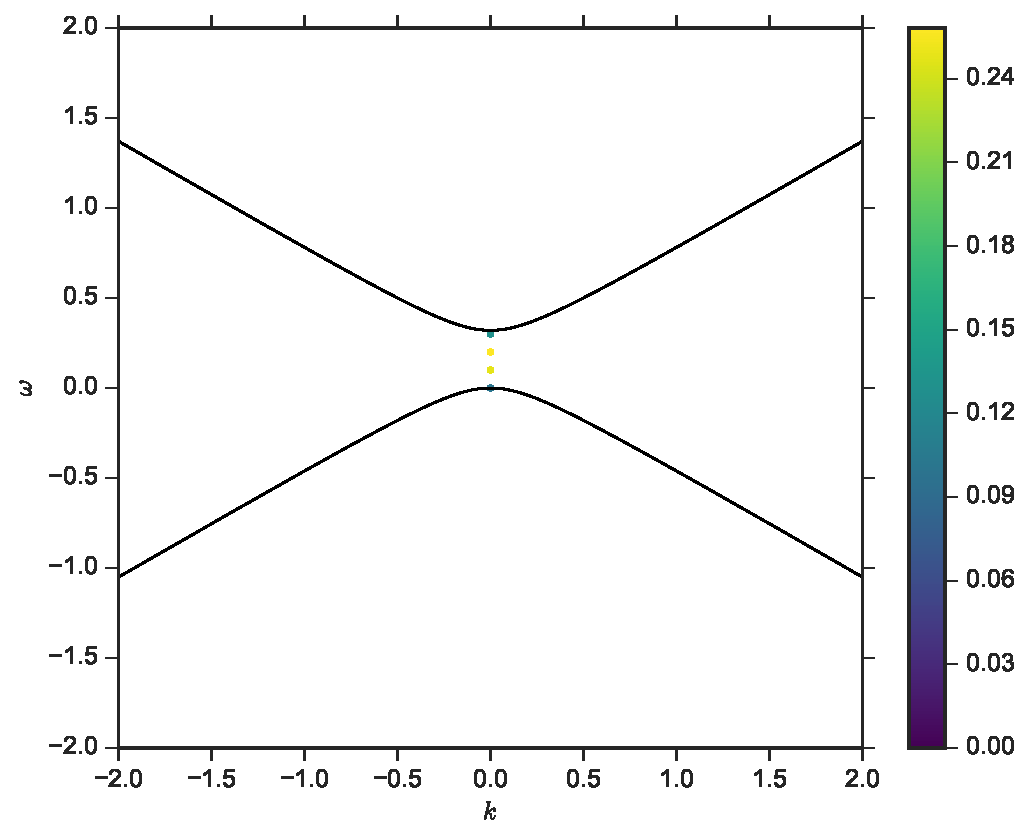
\includegraphics[width=\linewidth]{assets/spectDBWC1DRDBMAAPlt.pdf}
\endminipage\hfill
\minipage{0.32\textwidth}
  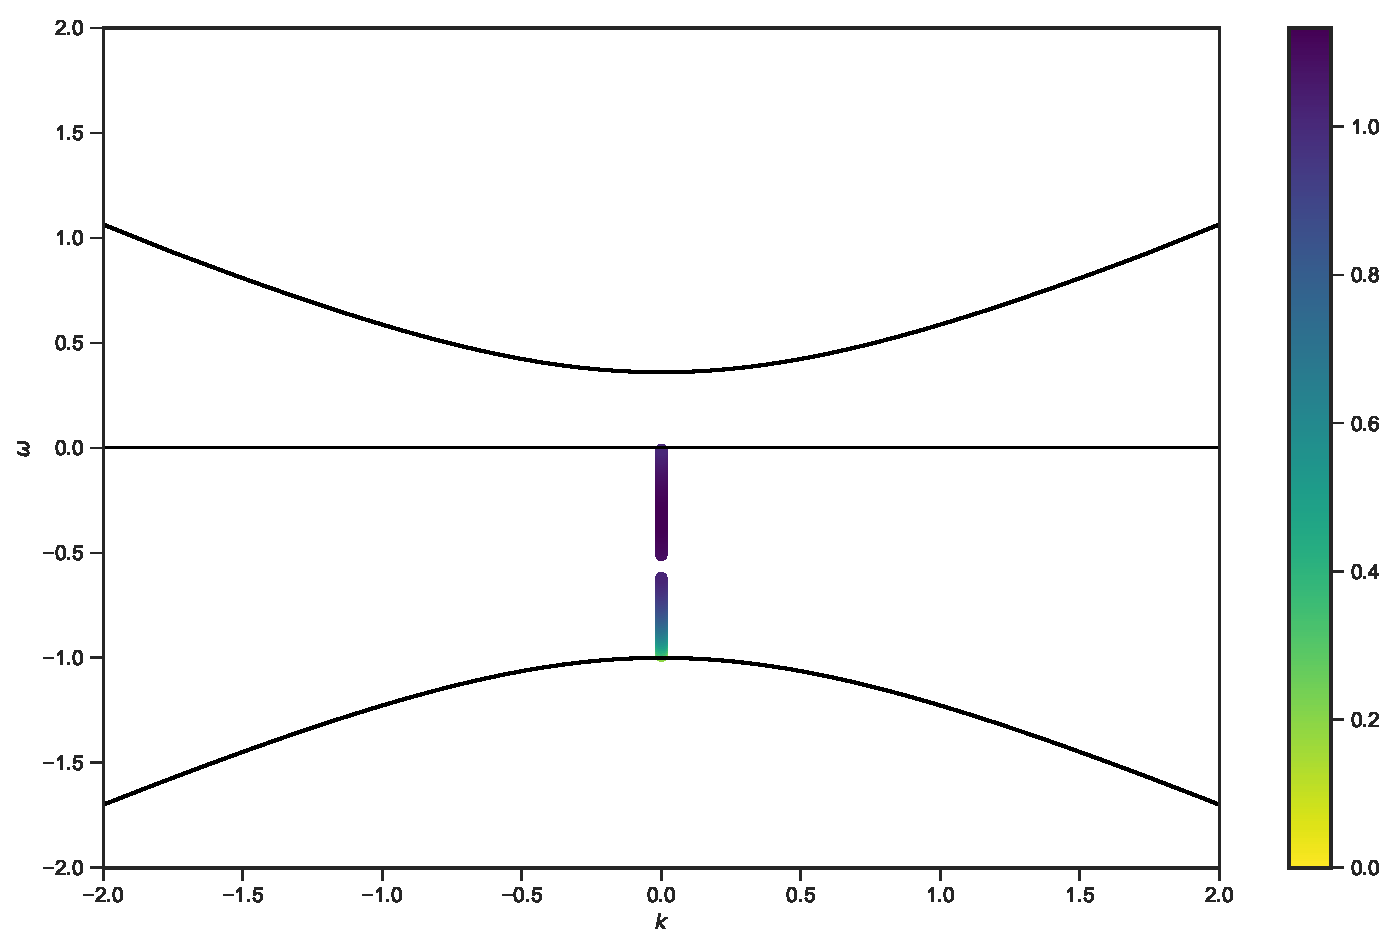
\includegraphics[width=\linewidth]{assets/spectDBWC1DRDBMZApPlt.pdf}
\endminipage\hfill
\minipage{0.32\textwidth}%
  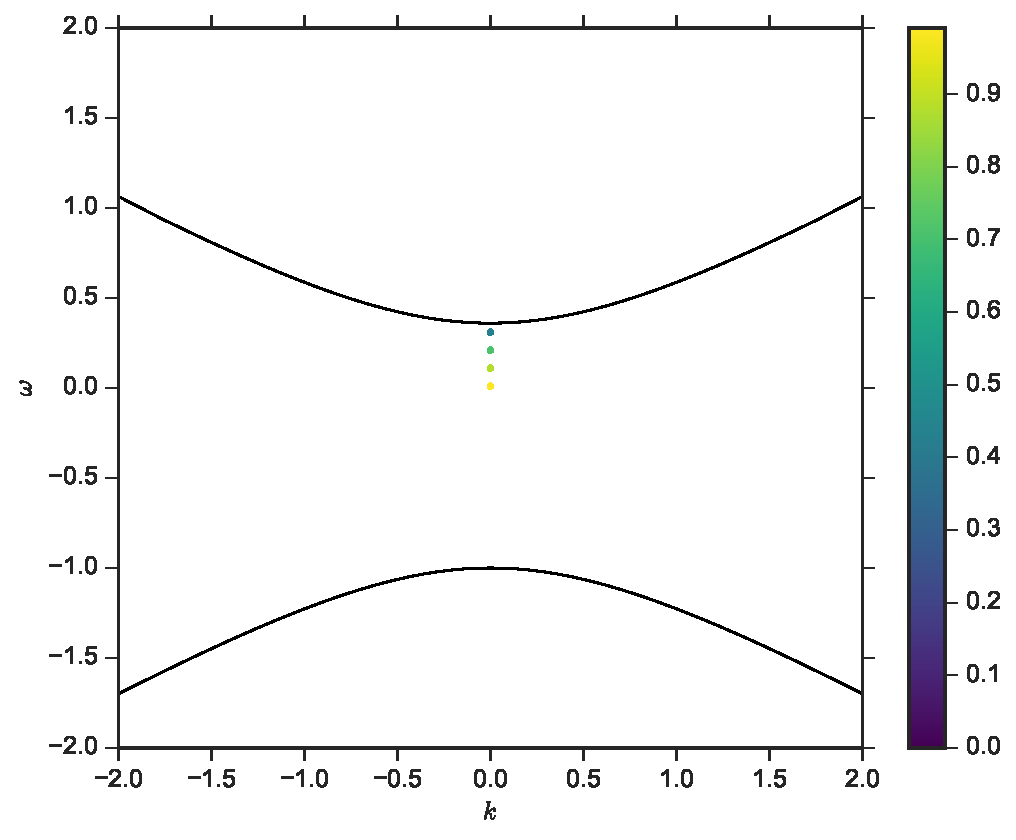
\includegraphics[width=\linewidth]{assets/spectDBWC1DRDBMZAmPlt.pdf}
\endminipage
\newline
\minipage{0.32\textwidth}
  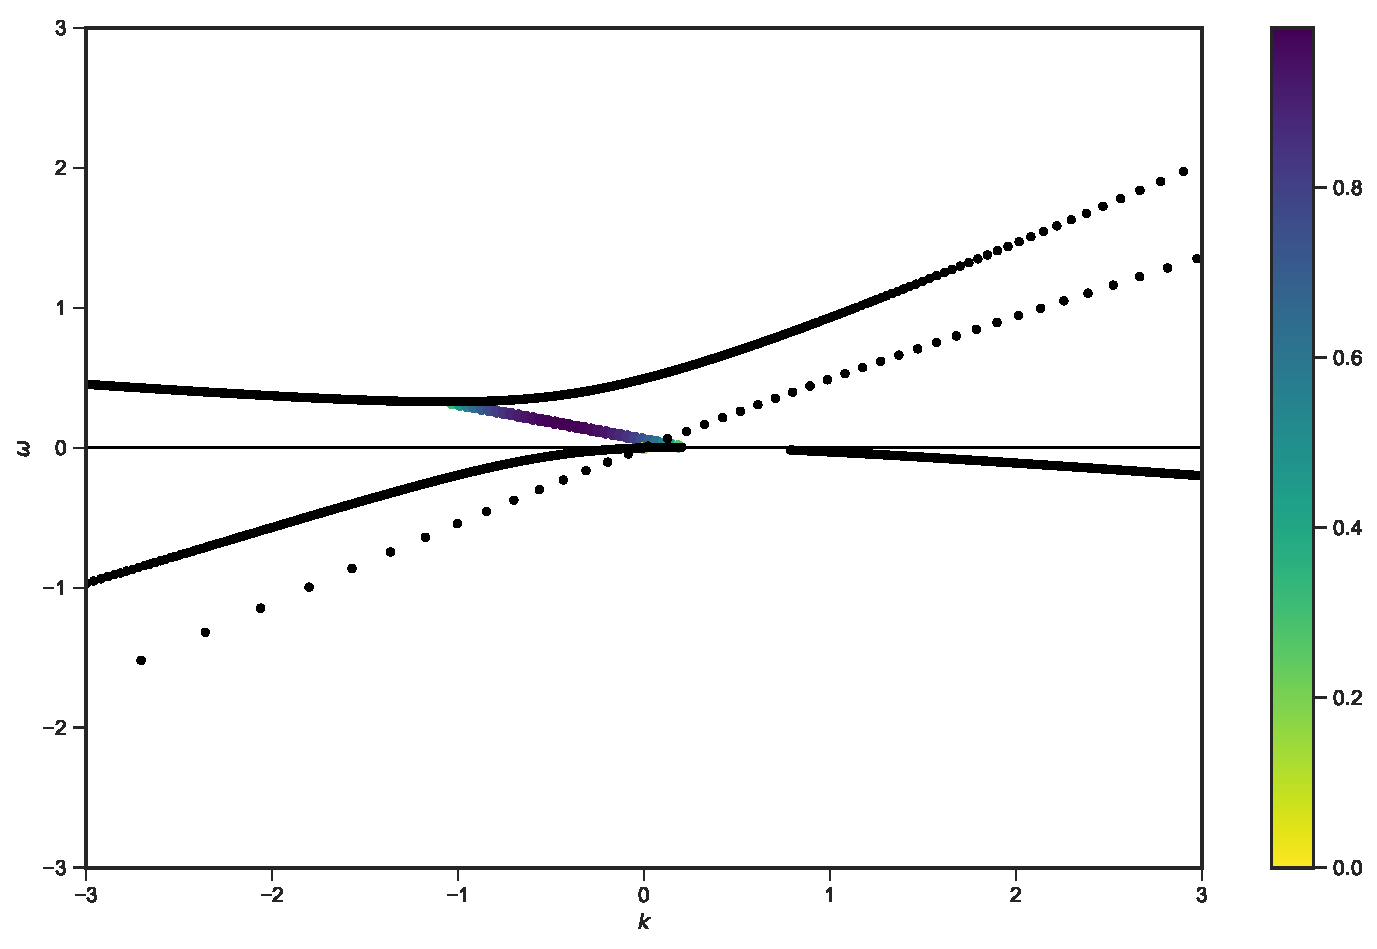
\includegraphics[width=\linewidth]{assets/spectDB3WC4DRDBMAAPlt.pdf}
\endminipage\hfill
\minipage{0.32\textwidth}
  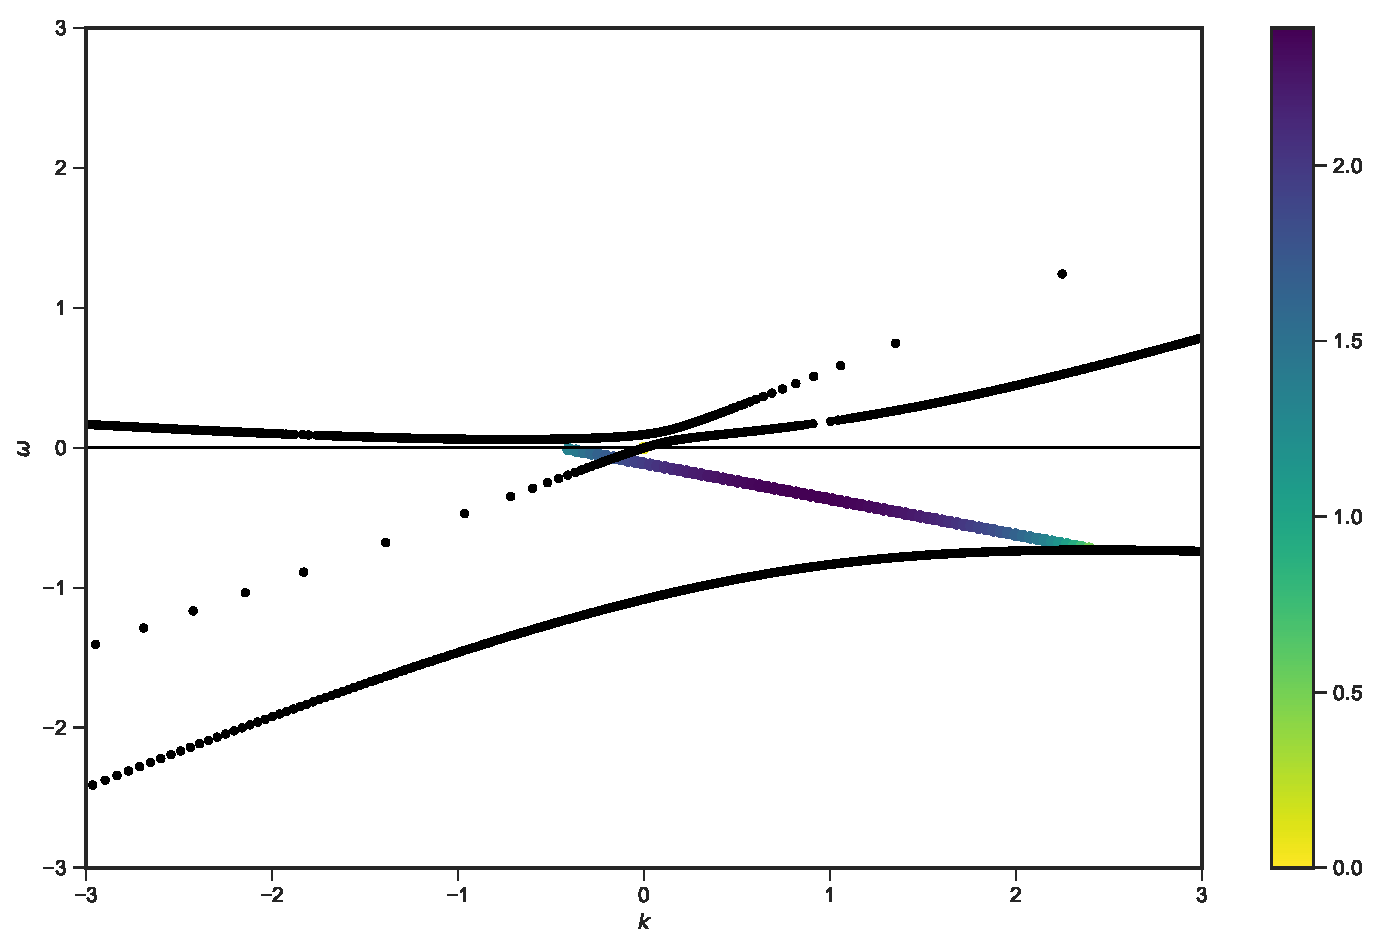
\includegraphics[width=\linewidth]{assets/spectDB3WC4DRDBMZApPlt.pdf}
\endminipage\hfill
\minipage{0.32\textwidth}
  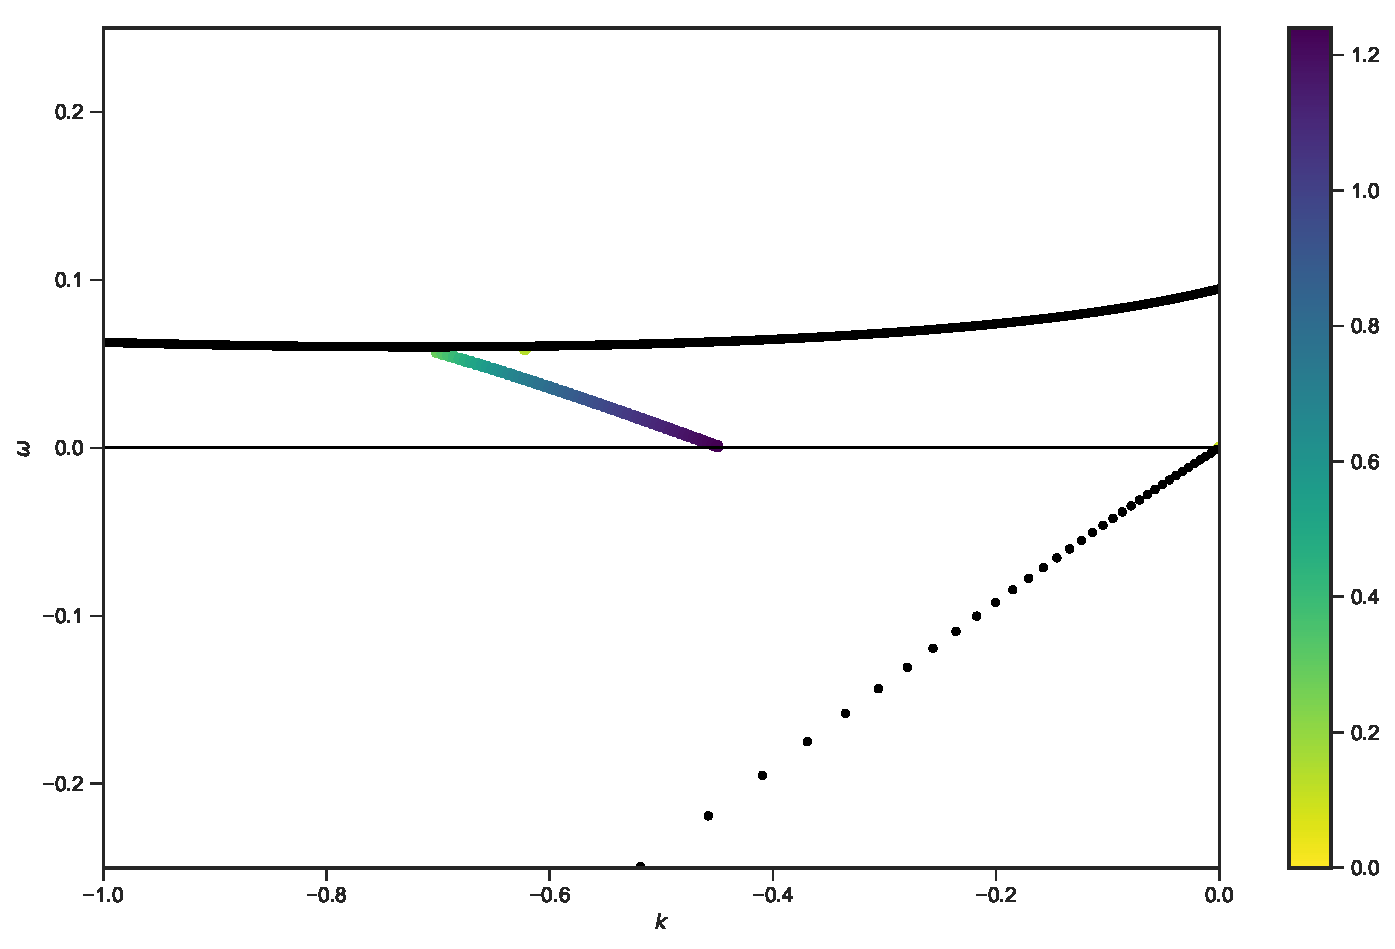
\includegraphics[width=\linewidth]{assets/spectDB3WC4DRDBMZAmPlt.pdf}
\endminipage\hfill
\caption{Dispersion relation and instabilities of two zenith angles spectrum (upper panels) and three zenith angles spectrum (lower panels). The black lines are the dispersion relations and the colored dots are examples of complex $\omega$ for real $k$. The left panels shows the dispersion relation and linear stability analysis of MAA solutions. The mid and right panels show the dispersion relation of MZA solutions.}
\label{fig-dr-db}
\end{figure}


However, this conclusion can not be generalized to arbitrary number of emission angles. As an example, we perform linear stability analysi of the three zenith angles emission configuration which is determined by a cubic function both in $\omega$ and $k$. Thus three solutions of $k$ ($\omega$) for given real $\omega$ ($k$) are epxected. As long as real solutions disappear, complex solutions emerge, which leads to instabilities occur even without an actual gap. As an example, we fix $\omega= 0.5$ for MAA solution (Fig. \ref{fig-dr-db} lower left panel). The three solutions of $k$ are $k=-4.6, 0.29, 1.2$.  $0.2$ which are all real and indicates no spatial instabilities. However, for another real $\omega = 0.2$, we find only one real solution $k=0.4$ from dispersion relation. The other solutions are complex and proven to be $k = -0.557106\pm 0.966535\mathrm i$ where the value with positive imaginary part leads to exponential growth. This gap and instability inconsistancy also exists in continuous angular distribution of neutrino emission.









{\color{red}\bf The forbidden region is determined by the emission angles. But is the forbidden region useful here? I don't think so.}

{\color{red}\bf I could show the results for C4 since it has both MAA and MZA instabilities. But we care about complex $k$ the most so I guess WC4 is fine.}

{\color{red}\bf Should I combine the MZA+ and MZA- solutions? }

{\color{red}\bf Font size in the plots are too small. But the font size depends on whether I need to combine MZA+ and MZA- solutions. }

{\color{red}\bf $\omega=0$ lines in the plots should be made distinguishable from the DR. }



\section{\label{sec-continuous-spectrum}Continuous Spectrum}

More realistic models of supernova explosions involves continuous zenith angle ELN spectra. In the earlier works of fast modes, Sawyer analyzed a box shaped angular distribution of neutrino emission \cite{Sawyer2016}. We show that the relation between instability and gap in dispersion relation breaks down for some box spectrum.

\subsection{\label{sec-boxspectrum}Box Spectra}

We construct a box spectrum with value $-0.1$ within $u\in [-1,-0.3)$ and value $1$ within $[-0.3,1]$ as shown in the top left panel of Fig. \ref{fig-box-c1}. With the spectrum defined, we calculate the dispersion relation and find out complex values of $k$ for real $\omega$.


\begin{figure}
   \minipage{0.49\textwidth}
     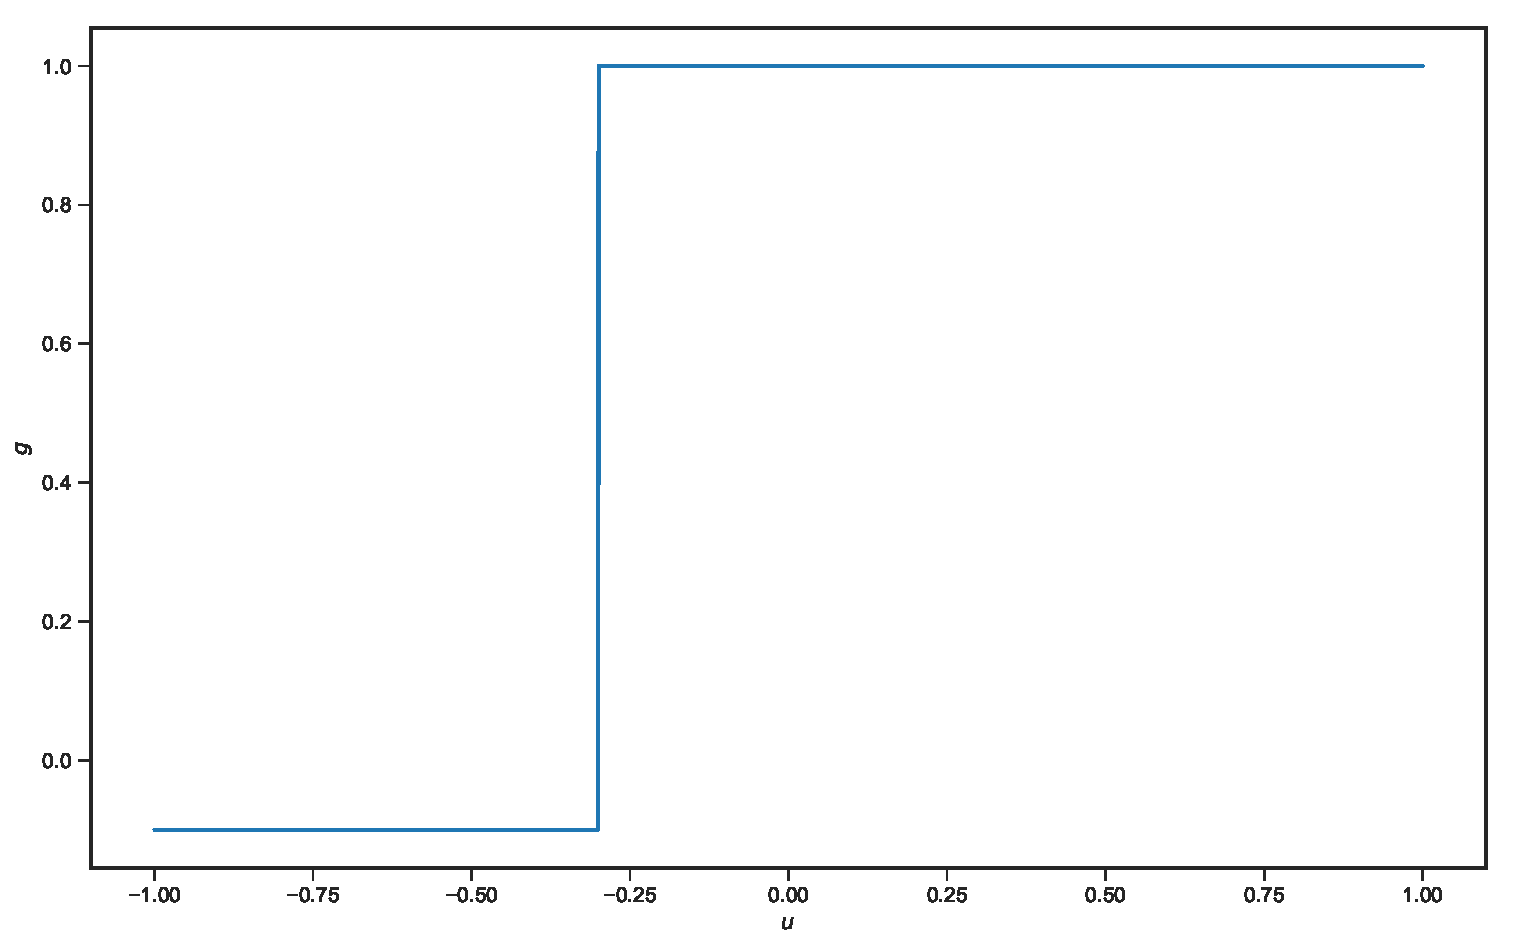
\includegraphics[width=\linewidth]{assets/spectBoxC1Spectrum.pdf}
   \endminipage\hfill
   \minipage{0.49\textwidth}
   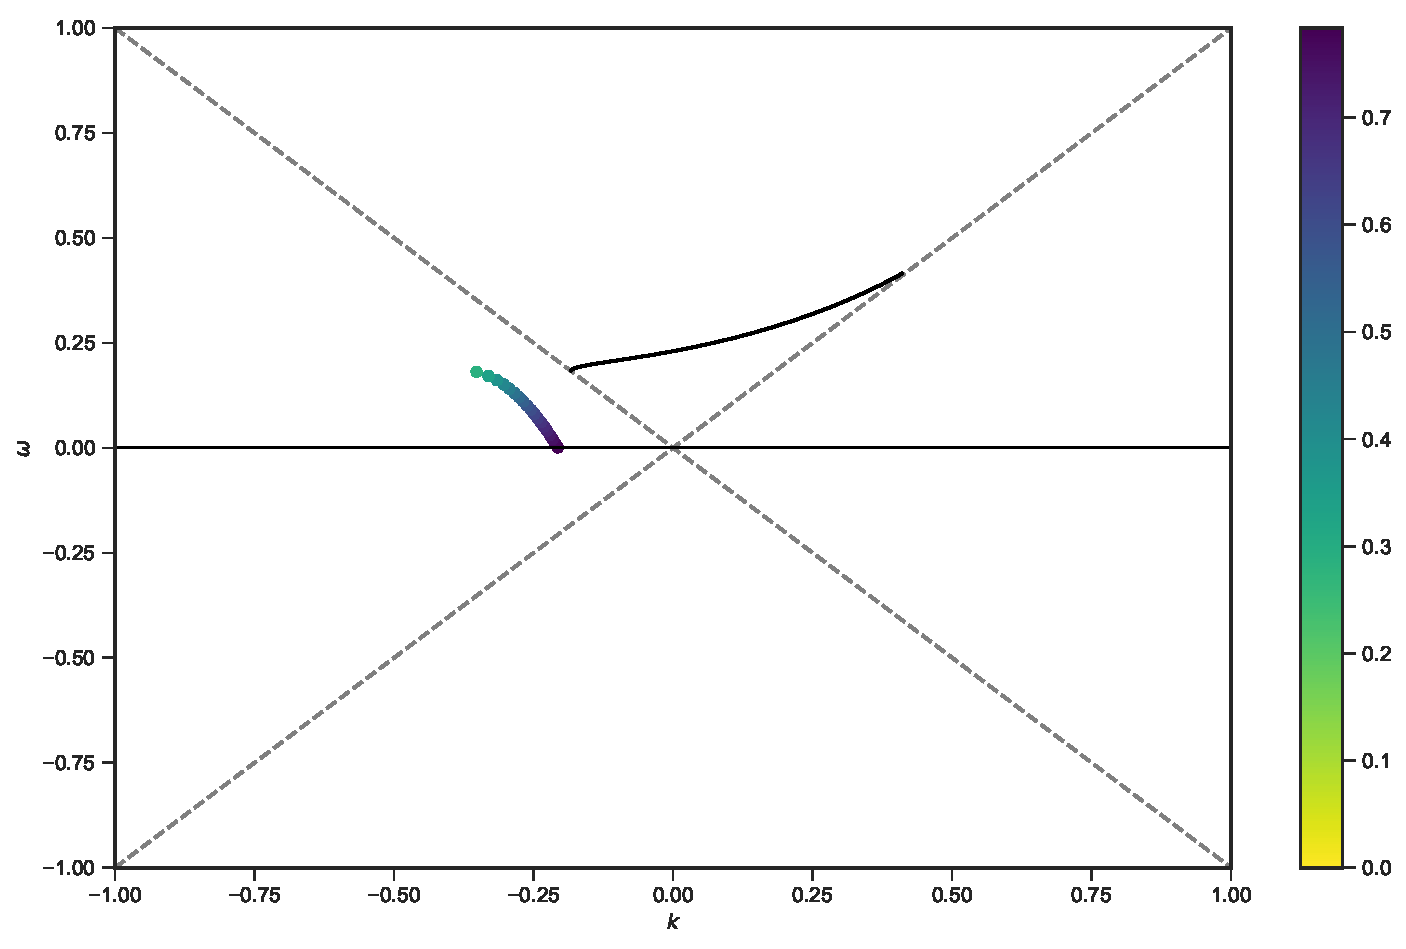
\includegraphics[width=\linewidth]{assets/spectBoxC1MAADRPlt.pdf}
   \endminipage\hfill
   \minipage{0.49\textwidth}
   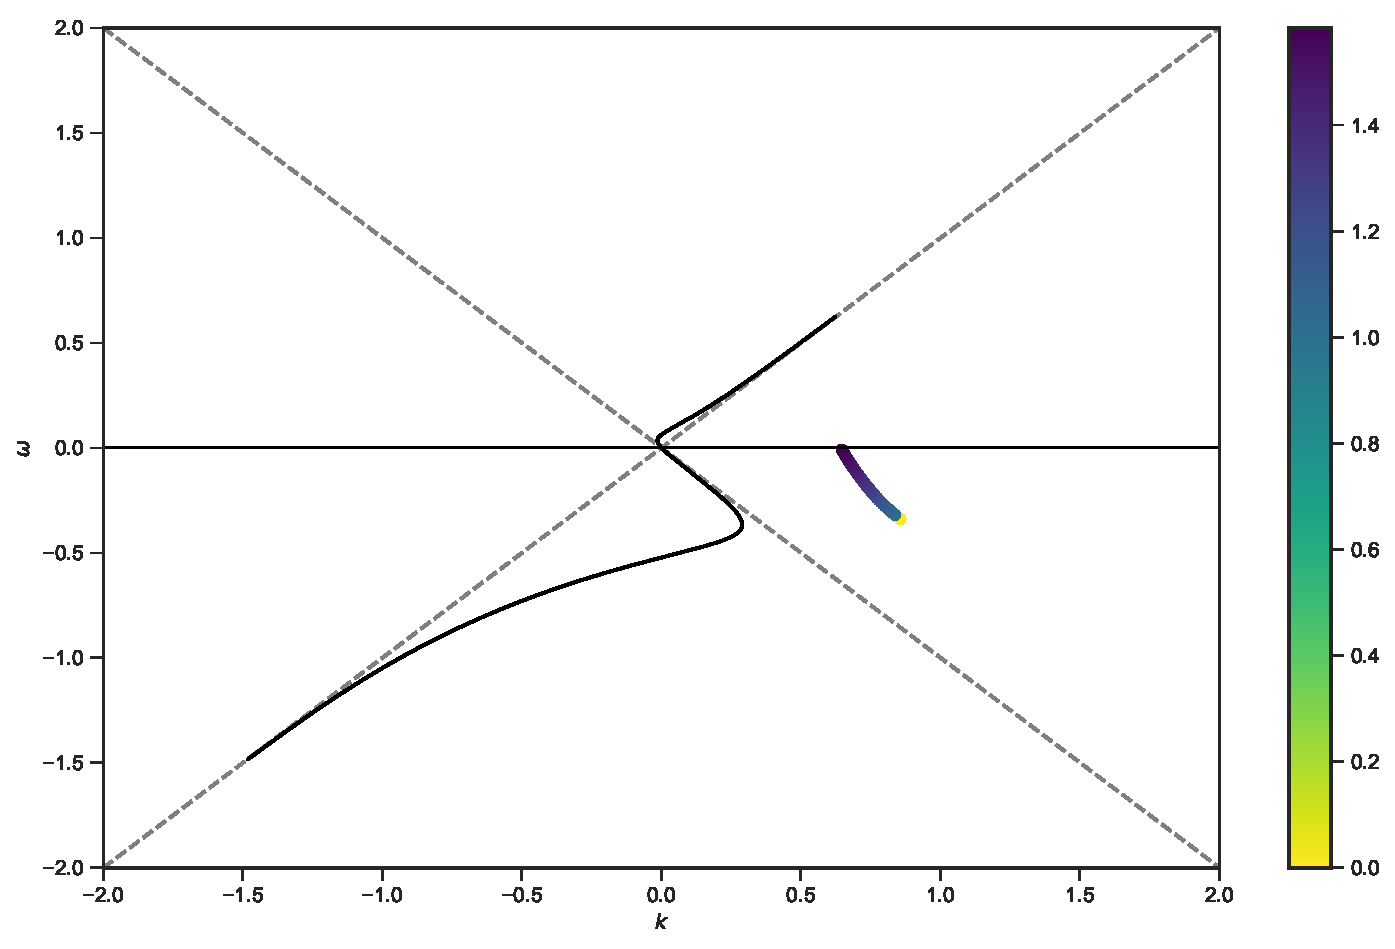
\includegraphics[width=\linewidth]{assets/spectBoxC1MZApDRPlt.pdf}
   \endminipage\hfill
   \minipage{0.49\textwidth}
   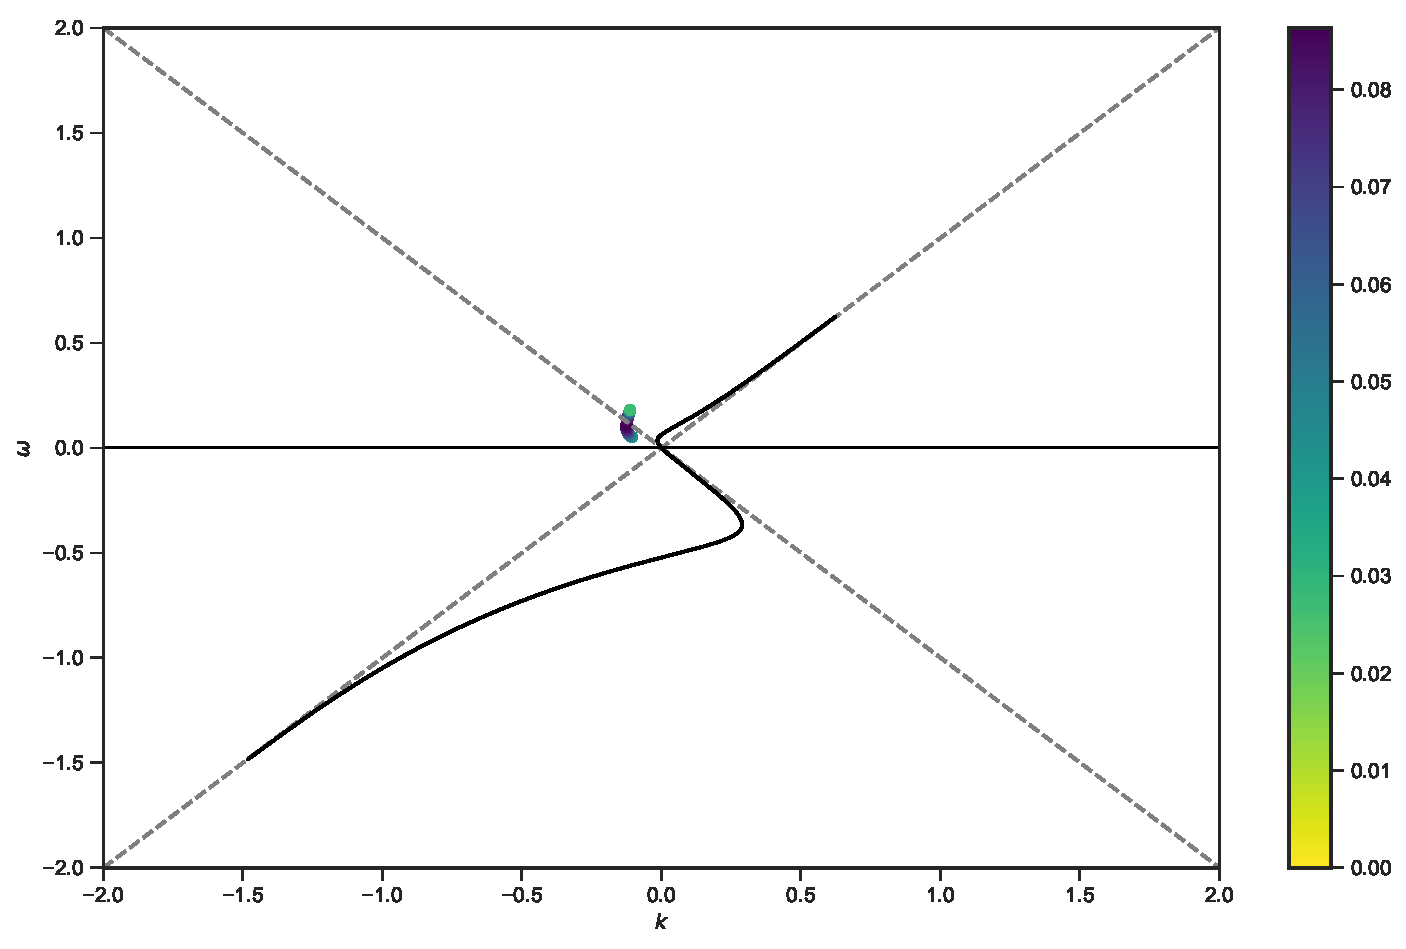
\includegraphics[width=\linewidth]{assets/spectBoxC1MZAmDRPlt.pdf}
   \endminipage\hfill
   \caption{Dispersion relation and linear stability analysis for box spectrum. The box spectrum is defined to be $-0.1$ within range $u\in [-1,-0.3)$ and $1$ within range $u\in [-0.3,1]$ as shown in the top left panel. The top right panel shows the dispersion relation and the complex $k$ for real $\omega$ for MAA solution. The lower panels shows the dispersion relation and complex $k$ for real $\omega$ for MZA solutions. Dashed gray lines are lines of $\omega= \pm k$ which sets the boundaries of the forbidden region for dispersion relation.
    }
   \label{fig-box-c1}
\end{figure}


\subsection{\label{sec-linear-spectrum}Linear Spectrum}


To address the fact that instability does not always show up in dispersion relation as gap, we calculate the dispersion relation relation for a linear spectrum with crossing.


\subsection{\label{sec-garching}Garching 1D Simulation Spectrum}





\begin{figure}
   \minipage{0.49\textwidth}
     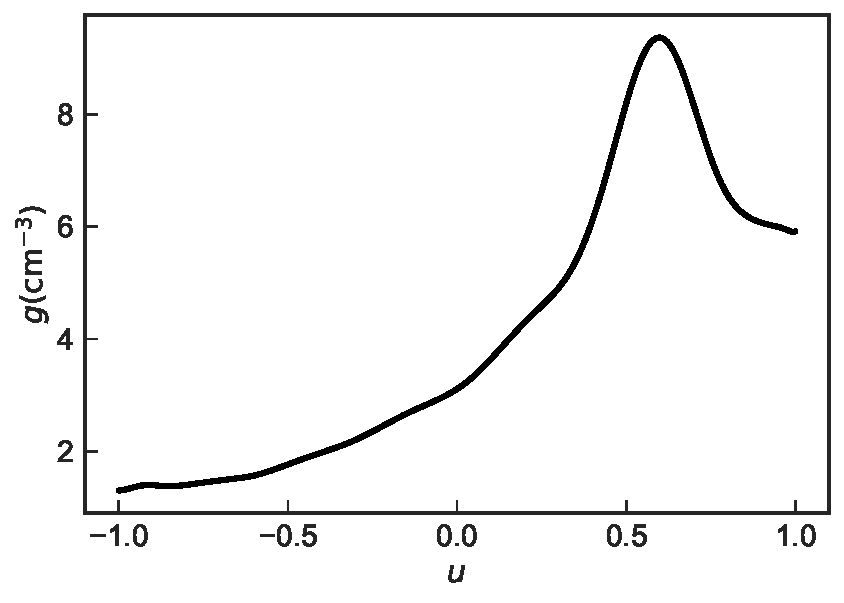
\includegraphics[width=\linewidth]{assets/spectGarchingPlt.pdf}
   \endminipage\hfill
   \minipage{0.49\textwidth}
   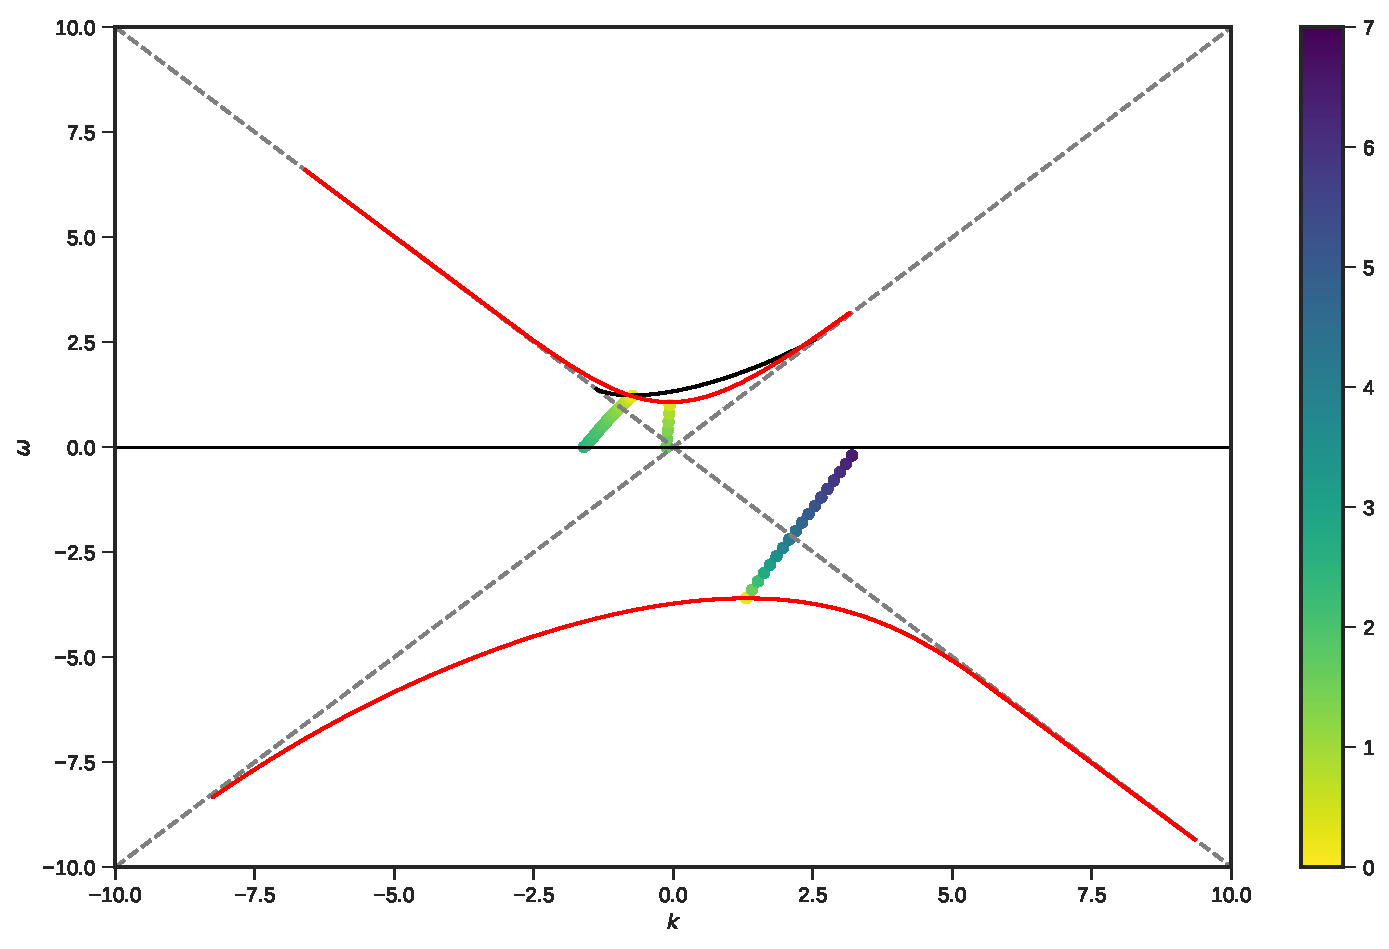
\includegraphics[width=\linewidth]{assets/spectGarchingDRLSAPlt.pdf}
   \endminipage\hfill
   \caption{Dispersion relation and linear stability analysis for a spectrum constructed from Garching 1D simulation data (left panel). From left to right, the sets of colored dots are the complex $k$ for MAA solution, MZA-, and MZA+ solutions respectively.
    }
   \label{fig-garching}
\end{figure}




\subsection{\label{sec-omega-to-zero}Instabilities at $\omega\to 0$}

\begin{equation}
   4 = \bar I_0 - \bar I_2
\end{equation}

\begin{equation}
   4 = \frac{1}{k} \int G(u) \frac{ 1 - u^2 }{ \omega/k - u }
\end{equation}

\begin{align}
k_R =& \frac{1}{4}\left(  \mathscr P \int G(u) \frac{ 1 - u^2 }{  - u }  \right) \\
k_I =&  \frac{\pi}{4}G(0) \operatorname{Sign}\left( \omega \right) \operatorname{Sign}\left(  \operatorname{Im}(k)  \right)
\end{align}


\begin{equation}
   \lvert k_I \rvert  =  \frac{\pi}{4}G(0) \operatorname{Sign}\left( \omega \right).
\end{equation}


\section{\label{sec-conclusion}Conclusion}






















%%%%%%%%%%%%%%%%%%%%%%%%%%%%%%%%%%%%%%%%%%%%%
%% APPENDIX
%%%%%%%%%%%%%%%%%%%%%%%%%%%%%%%%%%%%%%%%%%%%%

\appendix
\section{\label{sec-outline}Plan of the paper}



\begin{itemize}
    \item \sout{Review fast mode oscillations}
    \item \sout{State what has been done in Raffelt's paper.}
    \item \sout{The conclusion is not true.}
    \item \sout{Two zenith angles examples to prove that the number of solutions is the key.}
    \item \sout{Three zenith angles examples to show that not exactly related to gap.}
    \item Show that the continuous case is not related to gap at all. Box spectrum?
    \item Continuous spectrum or Garching group, data to show that we can prove the location of the instability.
    \item {\color{red}\bf Tweak the font size of plots.}
\end{itemize}


But I have a question. Is it really reliable? Should I use principal value integral for box spectrum DR?

We are still not crystal clear about the relation between gap and lsa.





\bibliographystyle{apsrev4-1}
\bibliography{ref.bib}

\end{document}
%
% ****** End of file apssamp.tex ******
